% =====================================================================
% Template LaTeX – Traces distribuées aux étudiants
% Auteur : (à compléter)
% Compilation : pdflatex/xelatex (pdflatex recommandé ici)
% =====================================================================
\documentclass[11pt,a4paper]{report}

% -------------------- Encodage & langue --------------------
\usepackage[T1]{fontenc}
\usepackage[utf8]{inputenc}
\usepackage[french]{babel}
\usepackage{lmodern}
\usepackage{microtype}
\usepackage{amsmath, amssymb}
\usepackage{multicol}
\usepackage{enumitem}

\usepackage{amsfonts}
\usepackage[version=4]{mhchem}
\usepackage{stmaryrd}
\usepackage{graphicx}
\usepackage[export]{adjustbox}
\graphicspath{ {./images/} }
\usepackage{caption}
\usepackage{multirow}

% -------------------- Mise en page --------------------------
\usepackage[a4paper,margin=2cm]{geometry}
\usepackage{fancyhdr}
\usepackage{parskip}      % espace entre paragraphes
\setlength{\parindent}{0pt}

% -------------------- Couleurs & liens ----------------------
\usepackage{xcolor}
\definecolor{Theme}{HTML}{0E7490} % teal-700
\definecolor{ThemeLight}{HTML}{E0F2F1}
\definecolor{Accent}{HTML}{F59E0B} % amber-500
\definecolor{Gray}{HTML}{374151}
\usepackage[colorlinks=true,linkcolor=Theme,urlcolor=Theme,citecolor=Theme]{hyperref}

% -------------------- Graphiques / décor --------------------
\usepackage{tikz}
\usetikzlibrary{patterns,positioning,calc}
\usepackage{graphicx}
\usepackage{tcolorbox}
\tcbuselibrary{skins,breakable,hooks,most}
\usepackage{fontawesome5}

% -------------------- Titres -------------------------------
\usepackage{titlesec}
\titleformat{\chapter}[display]
  {\Huge\bfseries\color{Theme}}
  {\filright\rule{0.75\linewidth}{1.2pt}\\[3pt]{Algèbre linéaire - Chapitre~\thechapter}}
  {0.2ex}
  {\filright}
  [\vspace{0.1ex}\rule{0.35\linewidth}{1.2pt}]

\titleformat{\section}
  {\Large\bfseries\color{Gray}}
  {\thesection}{0.6em}{}

% -------------------- En-têtes / pieds ---------------------
\pagestyle{fancy}
\fancyhf{}
\fancyhead[L]{\color{Gray}\leftmark}
\fancyhead[R]{\color{Gray}\textit{MEF - 2025/2026}}
\fancyfoot[R]{\color{Gray}\small p.\ \thepage}
\renewcommand{\headrulewidth}{0pt}
\renewcommand{\footrulewidth}{0pt}

% -------------------- Macros utilitaires -------------------


% Tcolorboxes stylisées
\tcbset{tracebox/.style={breakable,enhanced,sharp corners,boxrule=0pt,frame hidden,arc=2mm,
  colback=white,coltitle=black,fonttitle=\bfseries\large,
  borderline west={2mm}{0pt}{Theme},
  before skip=8pt,after skip=8pt,drop fuzzy shadow}}

\newtcolorbox{resumeBox}{tracebox,title={\faStickyNote\quad Résumé des idées}}
\newtcolorbox{rappelsBox}{tracebox,title={\faRedo\quad Ce que je dois savoir }}
\newtcolorbox{exempleBox}{tracebox,title={\faChalkboardTeacher\quad Exemple vu ensemble}}

% Encadré « Formules & illustrations »
\newtcolorbox{formulesBox}{tracebox,title={\faCalculator\quad Formules \& illustrations},colback=ThemeLight}

% Astuce : puces clean
\newenvironment{niceitemize}{\begin{itemize}\setlength{\itemsep}{0.25em}\color{Gray}}{\end{itemize}}

% Raccourci pour une « Trace » complète
% Usage : \TraceSection{Titre}{Objectif court}
\newcommand{\TraceSection}[2]{%
  
}

% -------------------- Page de titre ------------------------
\title{\textbf{Traces de cours}\\\large (résumés, formules, exemples, mini-exercices)}
\author{ MEF - 2025/2026 }
\date{\today}


\makeatletter
\renewcommand{\thesubsection}{\arabic{subsection}}
\renewcommand{\p@subsection}{}% supprime le préfixe section/chapter dans \ref
% Si vous voulez la même chose pour les sous-sous-sections :
% \renewcommand{\thesubsubsection}{\arabic{subsubsection}}
% \renewcommand{\p@subsubsection}{}
\makeatother

\usepackage{mdframed}
\usepackage{ifthen}

% \usepackage[sf]{titlesec}
% Définition de la variable pour afficher les corrections
\newboolean{showSolutions}
% Décommentez la ligne suivante pour afficher les solutions
\input \jobname.adr
% -------------------- Document ----------------------------
\begin{document}

\begin{center}
    {\LARGE \textbf{Méthode des éléments finis -- TD1}}\\[1em]
    {\large \textit{Librement inspiré de M. Jocelin Poulain}}
\end{center}
\captionsetup{singlelinecheck=false}
\section*{Problème}
On considère une barre de longueur $2 L$, constituée de deux barres de longueur égale :

\begin{itemize}
  \item Barre $AB$ (acier) : $L=6 \mathrm{~m}, \, E_{1}=210000 \mathrm{MPa},\,  A_{1}=0.001 \mathrm{~m}^{2}$
  \item Barre $BC$ (aluminium) : $L=6 \mathrm{~m}, \, E_{2}=70000 \mathrm{MPa},\, A_{2}=0.003 \mathrm{~m}^{2}$
\end{itemize}

(Remarquez que $E_1A_1 = E_2A_2$)

La barre $1$ est soumise à un chargement constant $p=100 \mathrm{kN} / \mathrm{m}$.

\begin{center}
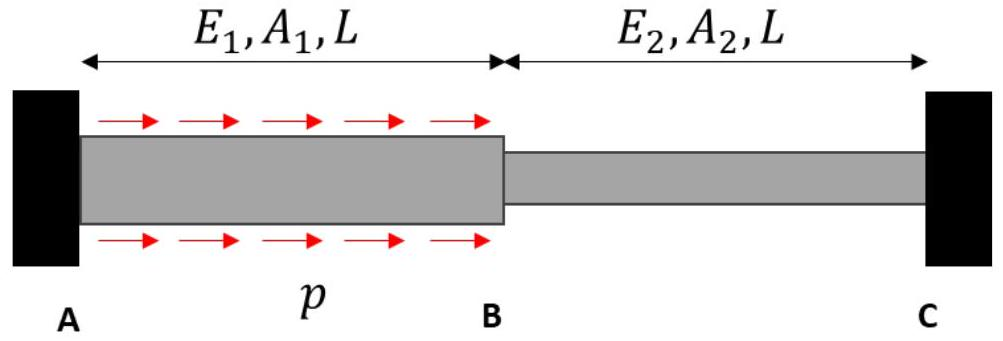
\includegraphics[max width=0.8\textwidth, center]{2025_10_03_26e11264345fd9bad5cag-1(2)}
\end{center}

On cherche à déterminer les contraintes et déformations dans la barre en résolvant d'une part le problème de manière exacte par les lois de l'élasticité et d'autre part par la méthode des éléments finis.

\section*{Partie 1 : Résolution par les lois de l'élasticité.}
La convention adoptée ici pour la loi de Hooke est : $\sigma=-E \varepsilon$ (convention Génie civil) On note $X_{1}$ la réaction à gauche et $X_{5}$ la réaction à droite.

\begin{enumerate}
  \item Déterminer l'expression de l'effort normal dans la barre en fonction de $X_{1}, p$ et de l'abscisse $x$.
  \ifthenelse{\boolean{showSolutions}}{
    \vspace{1em}
    \begin{mdframed}
      En procédant à une coupure à gauche d'une section $\Sigma(\mathrm{x})$, il vient :

      \begin{itemize}
        \item Pour $x<L$ : $N(x)=X_{1}+px$
          \begin{center}
          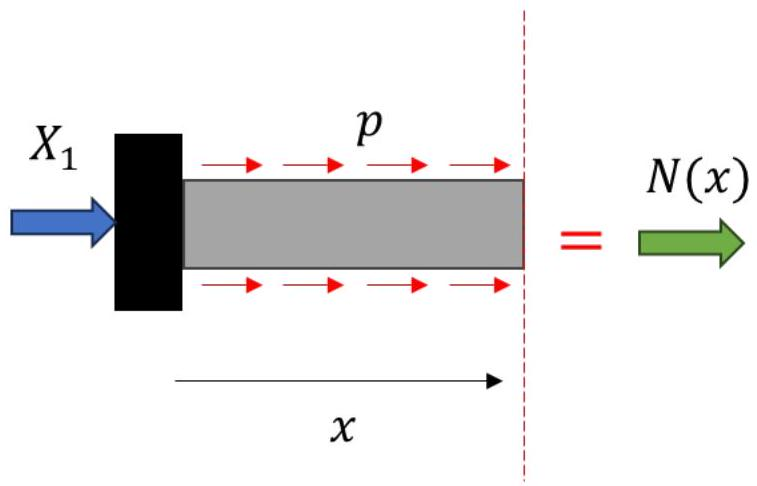
\includegraphics[width=0.6\textwidth]{2025_10_03_26e11264345fd9bad5cag-3}
          \end{center}
        \item Pour $x>L$ : $N(x)=X_{1}+p L$
      \end{itemize}
    \end{mdframed}
  }{}
  \vspace{1em}
  
  \item Déterminer l'allongement de la barre noté $u(x)$. Quelles sont les conditions aux limites ? En exploitant ces conditions aux limites, déterminer les réactions $X_{1}$ et $X_{5}$

  \ifthenelse{\boolean{showSolutions}}{
    \vspace{1em}
    \begin{mdframed}
      D'après la loi de Hooke :

      $$
      \varepsilon(x)=\frac{d u(x)}{d x}=-\frac{\sigma(x)}{E(x)}=-\frac{N(x)}{E(x) A(x)}
      $$

      On en déduit alors la translation horizontale des sections à une abscisse $x$ donnée :

      \begin{itemize}
        \item Pour $x<L$ : on est dans la $1^{\text {ère }}$ barre en acier :
      \end{itemize}

      $$
      u(x)=u_{A}-\int_{0}^{x} \frac{N(\xi)}{E_{1} A_{1}} d \xi=u_{A}-\int_{0}^{x} \frac{X_{1}+p \xi}{E_{1} A_{1}} d \xi=u_{A}-\frac{1}{E_{1} A_{1}}\left(X_{1} x+\frac{p x^{2}}{2}\right)
      $$

      On pourra noter que le déplacement en $\mathrm{x}=\mathrm{L}$ vaut alors :

      $$
      u(L)=u_{B}=u_{A}-\frac{1}{E_{1} A_{1}}\left(X_{1} L+\frac{p L^{2}}{2}\right)
      $$

      \begin{itemize}
        \item Pour $\mathrm{x}>\mathrm{L}$, on est dans la $2^{\text {nde }}$ barre en aluminium et l'effort normal est constant :
      \end{itemize}

      En se mettant dans le repère local de la seconde barre ( $x=0$ au début de la $2^{\text {nde }}$ barre), il vient :

      \begin{align*}
      u^{\prime}(x)& =u_{B}-\int_{0}^{x} \frac{N(\xi)}{E_{2} A_{2}} d \xi\\
       & =u_{B}-\int_{0}^{x} \frac{X_{1}+p L}{E_{2} A_{2}} d \xi\\
       & =u_{A}-\frac{1}{E_{1} A_{1}}\left(X_{1} L+\frac{p L^{2}}{2}\right)-\frac{1}{E_{2} A_{2}}\left(X_{1} x+p L x\right)
      \end{align*}

      Le déplacement de l'extrémité de la seconde barre vaut alors :

      $$
      u^{\prime}(L)=u_{C}=u_{A}-\frac{1}{E_{1} A_{1}}\left(X_{1} L+\frac{p L^{2}}{2}\right)-\frac{1}{E_{2} A_{2}}\left(X_{1} L+p L^{2}\right)
      $$

      Or, d'après les conditions aux limites : $u_{A}=u_{C}=0$\\
      On en déduit alors l'expression de la réaction $X_{1}$ :\\
      Soit :

      $$
      X_{1} L\left(\frac{1}{E_{1} A_{1}}+\frac{1}{E_{2} A_{2}}\right)+p L^{2}\left(\frac{\frac{1}{2}}{E_{1} A_{1}}+\frac{1}{E_{2} A_{2}}\right)=0
      $$

      On note que $E_{1} A_{1}=E_{2} A_{2}=E A=210 M N$. On en déduit alors :

      $$
      2 \frac{X_{1}}{E A}+\frac{3}{2}\frac{p L}{E A}=0
      $$

      Soit

      $$
      X_{1}=-\frac{3}{4} p L=- 0.75 * 100 * 6=-450 \mathrm{kN}
      $$

      On déduit également :

      $$
      X_{5}=-(p L+X_{1})=-\frac{p L}{4}=-150 \mathrm{kN}
      $$
    \end{mdframed}
  }{
  }
  \vspace{1em}

      Le champ de déplacement se déduit des équations de Bresse.\newline 

      Sur la page suivante est tracée l'allure du champ de déformation. 
      
      Il est parabolique sur la première partie de la barre et une linéaire sur la seconde partie. 
      
      On note que le déplacement maximal est obtenu en $x=4{,}5\,\mathrm{m}$, correspondant au point où $N(x)=0$ (séparation traction/compression).
      
      % Légère extension pour éviter un grand blanc si la figure déborde
      \enlargethispage{2\baselineskip}

      \begin{center}
      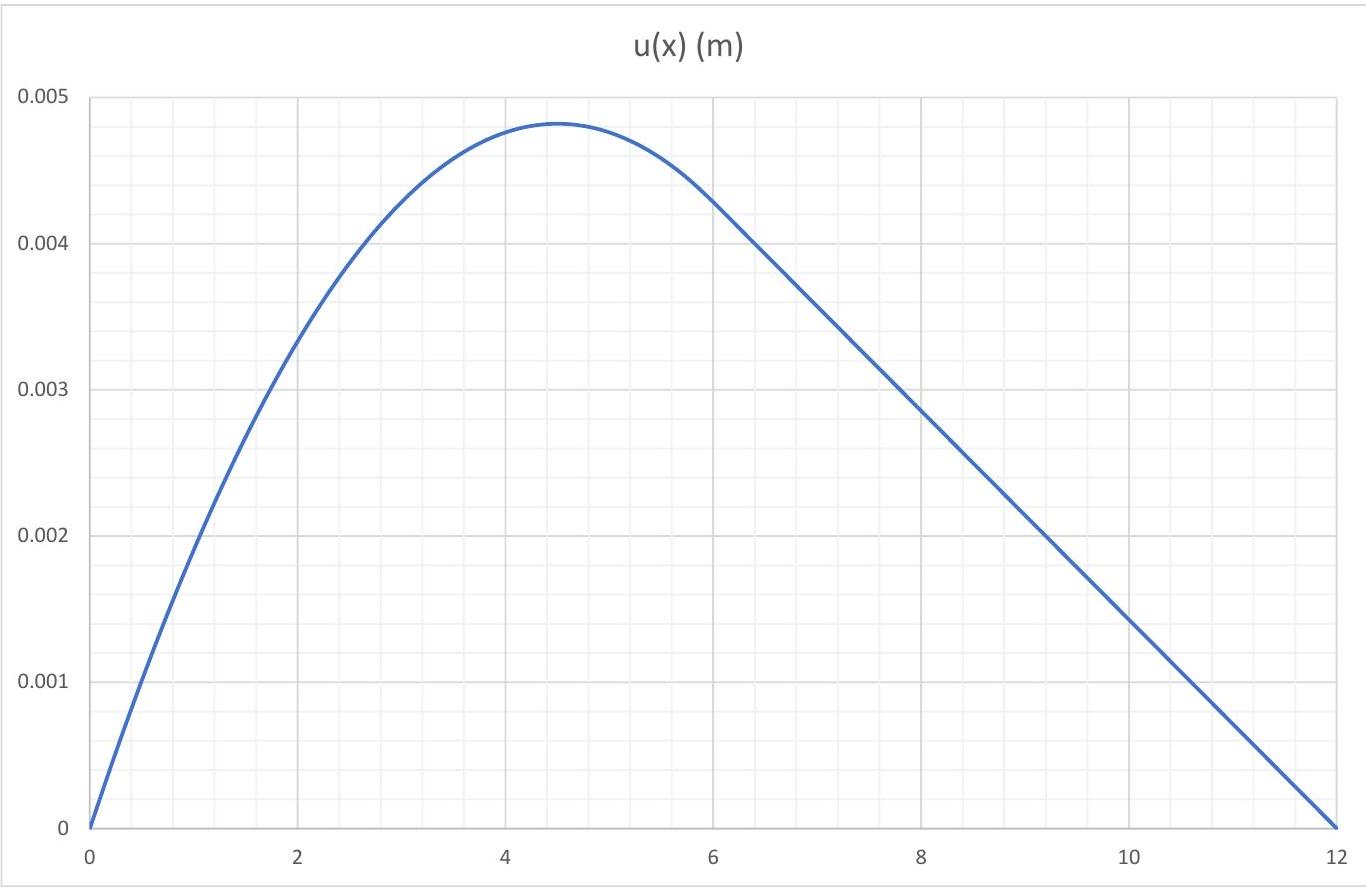
\includegraphics[width=0.8\textwidth]{2025_10_03_26e11264345fd9bad5cag-5}
      \end{center}
  
\end{enumerate}

\section*{Partie 2: Résolution par la MEF}
On utilise la méthode des éléments finis pour résoudre le problème (de manière approchée). On veut limiter la discrétisation à 4 éléments finis judicieusement choisis.

Comme vous le verrez, on retrouvera la solution exacte sur les nœuds du maillage, et on estimera la solution sur les autres points par interpolation.

\begin{enumerate}[start=6]
  \item Compte tenu des résultats précédents, préciser quel vous semble le meilleur maillage parmi les 3 présentés ci-dessous en justifiant votre choix :
\end{enumerate}

Maillage 1 : 
\begin{center}
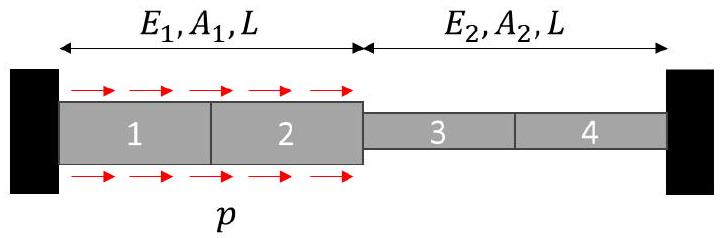
\includegraphics[width=0.7\textwidth]{2025_10_03_26e11264345fd9bad5cag-1(1)}
\end{center}

Maillage 2 :
\begin{center}
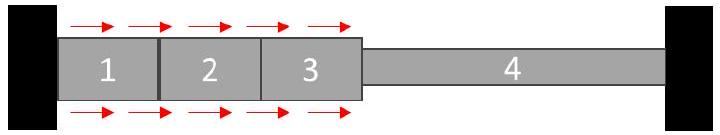
\includegraphics[width=0.7\textwidth]{2025_10_03_26e11264345fd9bad5cag-1}
\end{center}

Maillage 3 : 
\begin{center}
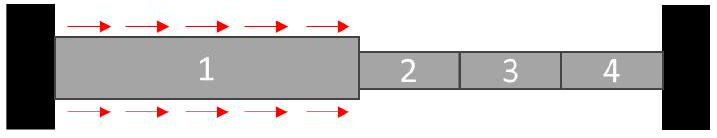
\includegraphics[width=0.7\textwidth]{2025_10_03_26e11264345fd9bad5cag-1(3)}
\end{center}




\ifthenelse{\boolean{showSolutions}}{
  \vspace{1em}
  \begin{mdframed}
    Il n'y a pas de chargement dans la seconde moitié de la barre : cette seconde moitié ne sera soumis qu'à des efforts à ses extrémités, à savoir la réaction d'appui de droite ( $X_{5}$ ) et l'effort provenant de la partie au niveau de la jonction entre les 2 moitiés ( $X_{B}$ ). 
    
    Les questions précédentes ont mis en évidence que la contrainte dans cette partie sont constantes. 
    Il n'est donc pas nécessaire de discrétiser cette seconde moitié. 
    
    En conséquence, le maillage 2 est le plus approprié car il permet une discrétisation de la première moitié de la poutre en 3 éléments et augmente donc ainsi la précision par rapport au maillage 1 ou au maillage 3.
  \end{mdframed}

\vspace{1em}

}{
}

\begin{enumerate}[start=7]
  \item La formule générale pour la matrice de rigidité d'un élément de barre est :

  $$
  K_e = \frac{EA}{L}
  \begin{bmatrix}
  1 & -1 \\
  -1 & 1
  \end{bmatrix}
  $$
  où $E$ est le module de Young, $A$ la section de l'élément, et $L$ sa longueur. 
  
  Pour le maillage choisi, déterminer les matrices de rigidités élémentaires. 

  \ifthenelse{\boolean{showSolutions}}{
    \vspace{1em}
    \begin{mdframed}
      On discrétise le $1^{\text {er }}$ tronçon en 3 éléments de 2 m et le second en un élément de 6 m .\\
      Les matrices de rigidité élémentaire de chacun des tronçons 1,2 et 3 valent ainsi :

      $$
      K_{1}=K_{2}=K_{3}=\frac{E A_{1}}{L_{1} / 3}\left[\begin{array}{cc}
      1 & -1 \\
      -1 & 1
      \end{array}\right]=\frac{3 E A_{1}}{L_{1}}\left[\begin{array}{cc}
      1 & -1 \\
      -1 & 1
      \end{array}\right]=105000\left[\begin{array}{cc}
      1 & -1 \\
      -1 & 1
      \end{array}\right](\mathrm{kN} / \mathrm{m})
      $$

      La matrice de rigidité élémentaire du tronçon 4 vaut ainsi :

      $$
      K_{4}=\frac{E A_{2}}{L_{2}}\left[\begin{array}{cc}
      1 & -1 \\
      -1 & 1
      \end{array}\right]=35000\left[\begin{array}{cc}
      1 & -1 \\
      -1 & 1
      \end{array}\right](\mathrm{kN} / \mathrm{m})
      $$

    \end{mdframed}

  \vspace{1em}
  }{
  }


  Pour écrire la matrice globale du système, il faut assembler les matrices de rigidité élémentaires de chaque barre en tenant compte de la connectivité des nœuds. On procède ainsi :

  \begin{itemize}
    \item Numéroter tous les nœuds du système.
    \item Partir d'une matrice carrée de dimension égale au nombre total de nœuds, remplie de zéros. La première ligne correspond au nœud 1, la deuxième au nœud 2, etc. de même pour les colonnes. 
    \item Pour chaque petit élément du maillage, identifier les nœuds à ses extrémités et le coefficient de la matrice élémentaire associé à ces nœuds.
    \item Dans la matrice globale, on additionne les contributions de chaque nœud à la position correspondante dans la matrice globale.
  \end{itemize}

  Mathématiquement, cela revient à superposer les matrices élémentaires dans la matrice globale en respectant la topologie du maillage.

  Par exemple, si un élément relie les noeuds 1 et 3, et que sa matrice élémentaire est :

  $$
  K_e = 
  \begin{bmatrix}
  a & b \\
  c & d
  \end{bmatrix}
  $$

  Alors, dans la matrice globale, cet élément contribuera aux positions (1,1), (1,3), (3,1) et (3,3):

  $$
  K = 
  \begin{bmatrix}
  a & . & b & \cdots  \\
  . & . & . & \cdots  \\
  c & . & d & \cdots \\
  \vdots & \vdots & \vdots & \ddots \\
  \end{bmatrix}
  $$
  \item Exprimer la matrice de raideur globale de la structure.

  \ifthenelse{\boolean{showSolutions}}{
    \vspace{1em}
    \begin{mdframed}

      La matrice de raideur est obtenue en procédant à l'assemblage des matrices élémentaires :

      $$
      K=\left[\begin{array}{ccccc}
      k_{1} & -k_{1} & 0 & 0 & 0 \\
      -k_{1} & k_{1}+k_{2} & -k_{2} & 0 & 0 \\
      0 & -k_{2} & k_{2}+k_{3} & -k_{3} & 0 \\
      0 & 0 & -k_{3} & k_{3}+k_{4} & -k_{4} \\
      0 & 0 & 0 & -k_{4} & k_{4}
      \end{array}\right]=\frac{EA}{L}\left[\begin{array}{lrcrr}
      3 & -3 & 0 & 0 & 0 \\
      -3 & 6 & -3 & 0 & 0 \\
      0 & -3 & 6 & -3 & 0 \\
      0 & 0 & -3 & 4 & -1 \\
      0 & 0 & 0 & -1 & 1
      \end{array}\right]
      $$
    \end{mdframed}
  }{
  }

  \vspace{1em}

  Pour écrire la relation $F=K \bf{u}$ et résoudre le système, il faut encore exprimer les forces qui s'appliquent sur les noeuds du maillage. \newline 
  Dans le cours de RdM, vous avez montré que le chargement réparti peut être remplacé par un chargement nodal équivalent $F_e = \frac{p L_e}{2}$.

  \item Déterminer les forces équivalentes qui s'appliquent sur les noeuds du maillage.

  \ifthenelse{\boolean{showSolutions}}{
    \vspace{1em}
    \begin{mdframed}
      Le chargement réel peut être remplacé par le chargement nodal équivalent :
      
      
      \begin{center}
        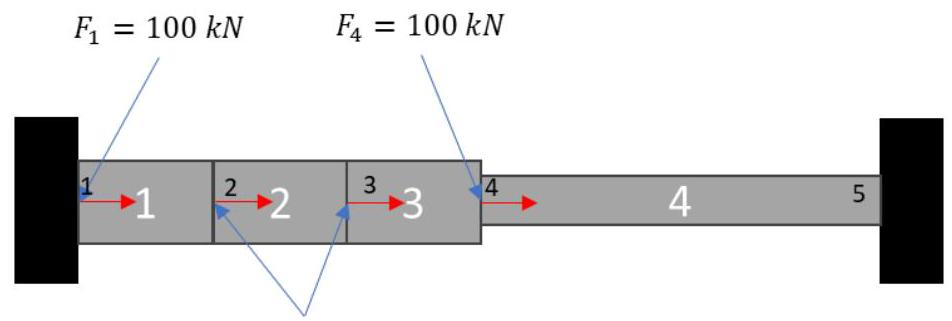
\includegraphics[width=0.8\textwidth]{2025_10_03_26e11264345fd9bad5cag-7}
      \end{center}
      
      $$
      F_{2}=F_{3}=200 \mathrm{kN}
      $$
      
      On vérifie que la résultante du chargement réel est bien identique à celle des forces nodales équivalentes, soit $600 \mathrm{kN}$.
    \end{mdframed}
    \vspace{1em}
  }{
  }



  Il reste une dernière étape avant d'écrire le système linéaire, il faut tenir compte des conditions aux limites. Pour cela, on supprime dans la matrice de rigidité globale les lignes et colonnes correspondant aux déplacements connus.

  \item Etablir la relation $F=K \bf{u}$ pour l'ensemble de la structure.

  \ifthenelse{\boolean{showSolutions}}{
    \vspace{1em}
    \begin{mdframed}
      On a supprimé les premières et dernières lignes et colonnes de la matrice de rigidité globale. Les conditions aux limites imposent $u_1 = u_5 = 0$.

      La relation force-déplacement de la structure est ainsi exprimée sous la forme matricielle :

      $$
      \begin{pmatrix}
        200 \\
        200 \\ 
        100 \\
      \end{pmatrix}
       = 
       \frac{EA}{L}\left[
        \begin{array}{lrcrr}
         6 & -3 & 0  \\
         -3 & 6 & -3  \\
         0 & -3 & 4  \\
        \end{array}\right]
        \begin{pmatrix}
          u_2 \\
          u_3 \\
          u_4 \\
        \end{pmatrix}
      $$
    \end{mdframed}

  \vspace{1em}
  }{
  }

  \item Ecrire puis résoudre le système linéaire pour obtenir les déplacements aux noeuds du maillage.

  \ifthenelse{\boolean{showSolutions}}{
    \vspace{1em}
    \begin{mdframed}
      On résout le système linéaire pour obtenir les déplacements.

    \[
    \left\{
    \begin{array}{rcl}
      6u_2 - 3u_3           & = & 200L/EA \\
      -3u_2 + 6u_3 - 3u_4   & = & 200L/EA \\
                -3u_3 + 4u_4 & = & 100L/EA \\
    \end{array}
    \right.
    \]

    Après l'opération $R_2 \leftarrow 2R_2 + R_1$, on obtient :

    \[
    \left\{
    \begin{array}{rcl}
      6u_2 - 3u_3           & = & 200L/EA \\
      9u_3 - 6u_4           & = & 600L/EA \\
      -3u_3 + 4u_4          & = & 100L/EA \\
    \end{array}
    \right.
    \]
    Ensuite, $R_3 \leftarrow 3R_3 + R_2$, ce qui donne le système suivant :

    \[
    \left\{
    \begin{array}{rcl}
      6u_2 - 3u_3           & = & 200L/EA \\
      9u_3 - 6u_4           & = & 600L/EA \\
      6u_4           & = & 900L/EA \\
    \end{array}
    \right.
    \]
    On obtient finalement :
    \[
    \left\{\begin{array}{rcl}
      u_2 & = & 350L/3EA \\
      u_3 & = & 500L/3EA \\
      u_4 & = & 150L/EA \\
    \end{array}\right.
    \]

    \end{mdframed}

  \vspace{1em}
  }{
  }

  \item Tracer ainsi le champ de déplacements obtenu par la FEM sur le schéma donné ci-dessus et comparer au champ exact.

  \ifthenelse{\boolean{showSolutions}}{
    \vspace{1em}
    \begin{mdframed}      
      
      Les déplacements FEM et exacts sont identiques aux niveaux des nœuds du maillage, à savoir en $x=0,2,4,6$ et $12\,\mathrm{m}$ .\\

      Le champ FEM est identique au champ exact dans la partie de barre non chargée. 

      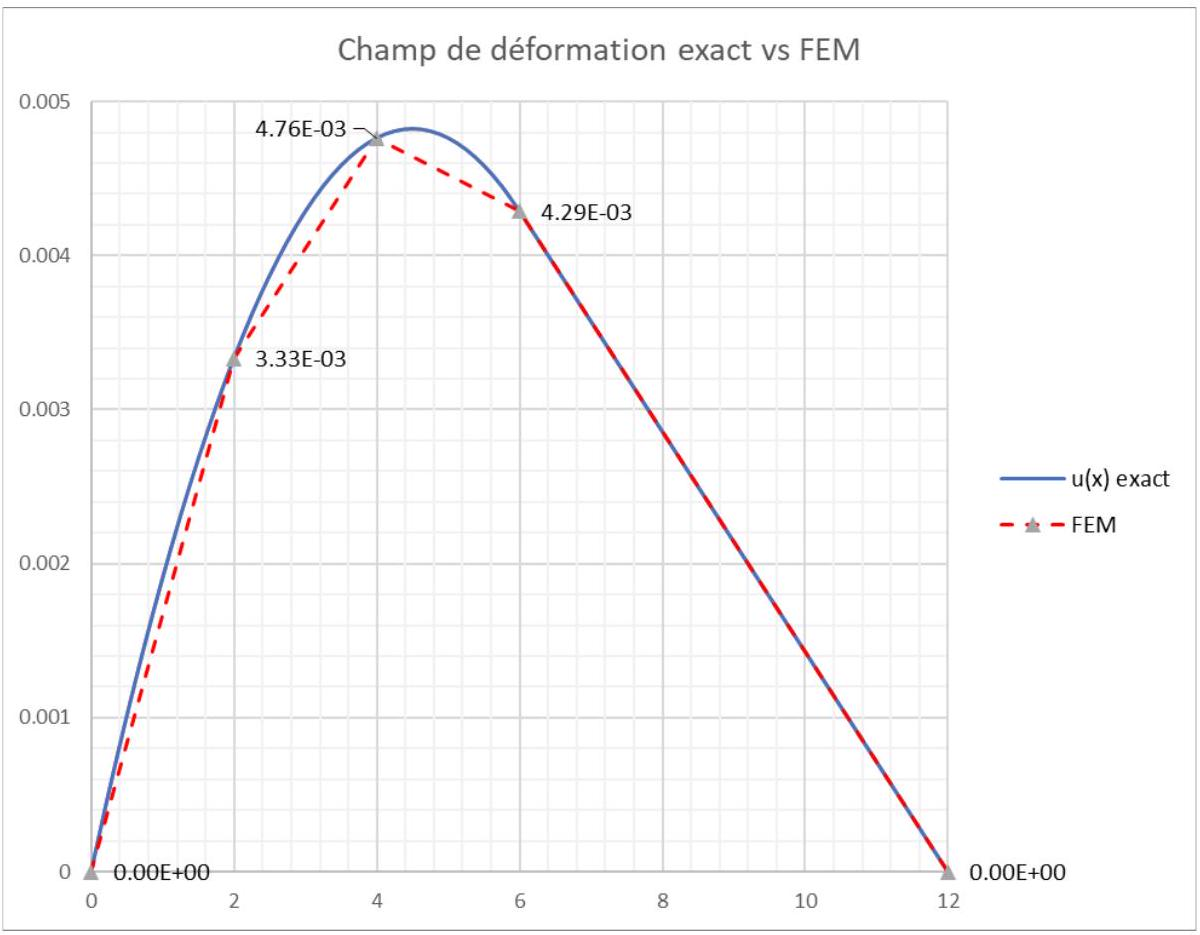
\includegraphics[max width=\textwidth, center]{2025_10_03_26e11264345fd9bad5cag-8}
      
      Il y a bien sûr un léger écart dans la partie de barre chargée. 

      Cet exemple montre aussi qu'un maillage « grossier » peut aboutir à une sous-estimation des contraintes.    
    \end{mdframed}
  }{
  }
\end{enumerate}

\end{document}